\documentclass[border=1cm,tikz]{standalone}
\usepackage{amsmath}

\usetikzlibrary{arrows.meta}
\usetikzlibrary{fadings}
\usetikzlibrary{decorations.markings}

\definecolor{lightblue}{rgb}{0.149,0.545,0.824}
\definecolor{darkblue}{rgb}{0.000, 0.275, 0.545}
\definecolor{darkred}{rgb}{0.647,0.129,0.149}
\definecolor{green}{rgb}{0.365, 0.592, 0.157}

\begin{document}

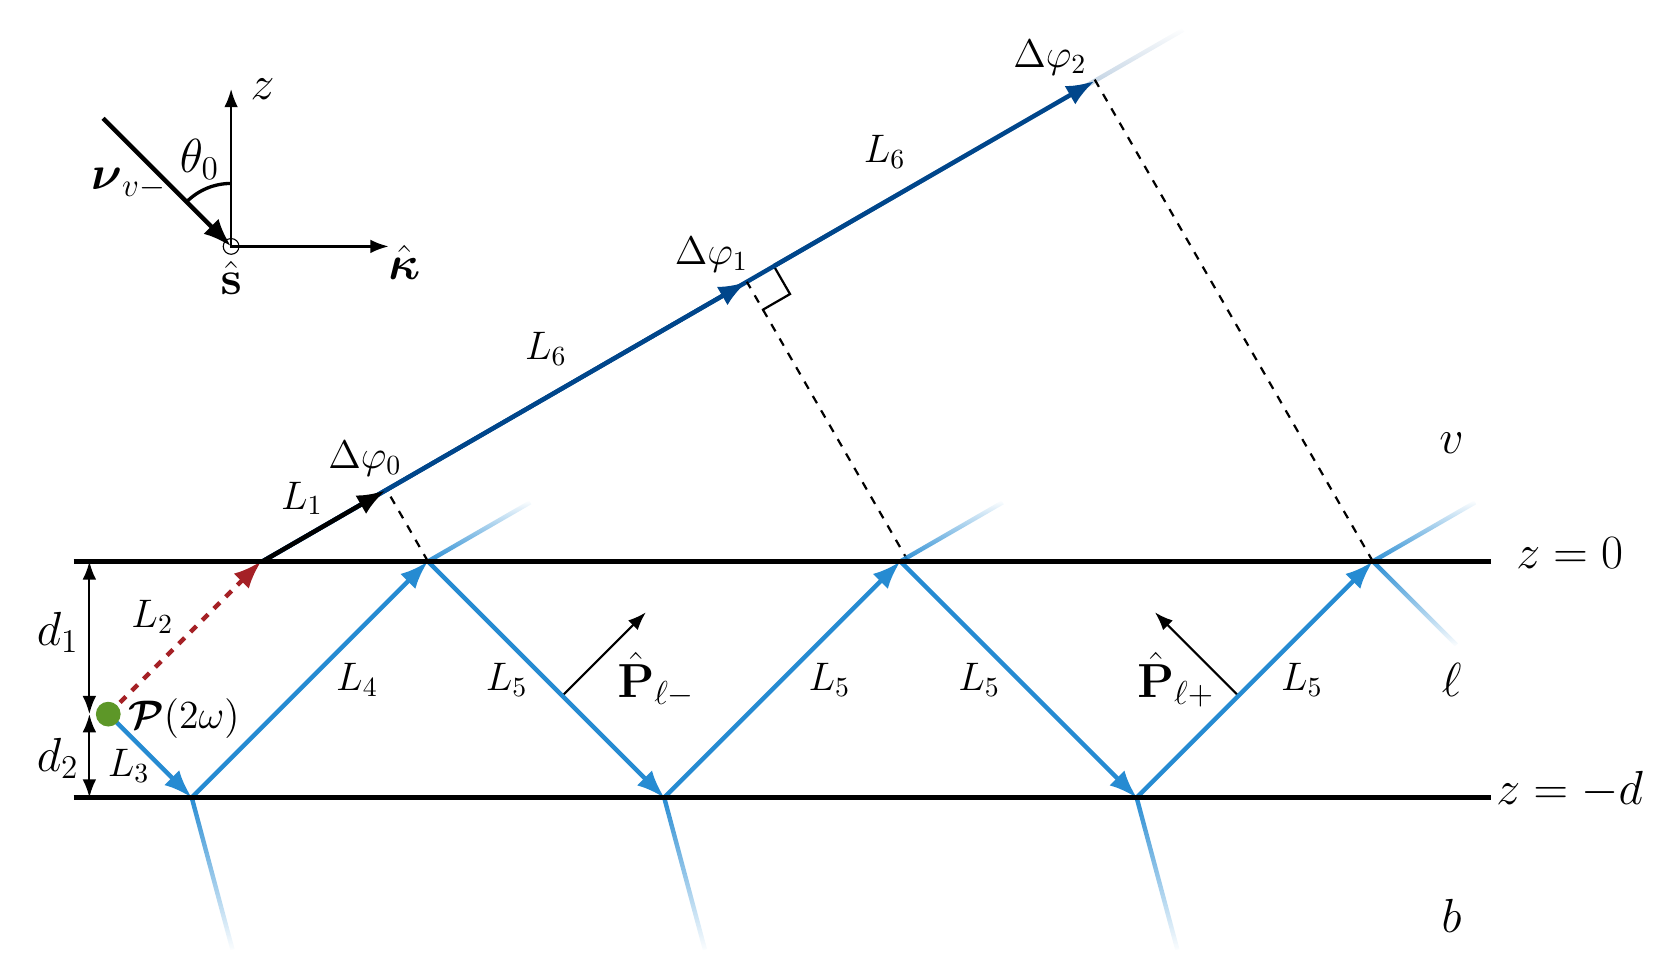
\begin{tikzpicture}

%% axes
\draw [very thick] (2,9) +(90:0.8) arc (90:135:0.8);
\draw [Latex-Latex,thick] (2,11) -- ++(0,-2) -- ++(2,0);
\draw [Latex-,ultra thick] (2,9) -- ++(135:2.3);
\draw [color=black] (2,9) circle (0.10);
\node at (1.6,10.1) {\LARGE $\theta_{0}$};
\node at (0.7,9.8) {\LARGE $\boldsymbol{\nu}_{v-}$};
\node at (2.4,11) {\LARGE $z$};
\node at (2,8.6) {\LARGE $\hat{\mathbf{s}}$};
\node at (4.2,8.8) {\LARGE $\hat{\boldsymbol{\kappa}}$};

%% outside
% arrows
\draw [thick] (8.893,8.75) -- ++(-60:0.41) -- ++(-150:0.41); % right angle
\draw [ultra thick,darkblue,path fading=north] (8.893,8.75) -- ++(30:6);
\draw [-Latex,ultra thick,darkblue] (2.4,5) -- ++(30:12.2);
\draw [-Latex,ultra thick,darkblue] (2.4,5) -- ++(30:7.1);
\draw [-Latex,ultra thick] (2.4,5) -- ++(30:1.8);
% labels
\node at (2.9,5.8)   {\Large $L_{1}$};
\node at (6,7.7)     {\Large $L_{6}$};
\node at (10.3,10.2) {\Large $L_{6}$};
\node at (3.7,6.3)   {\Large $\Delta\varphi_{0}$};
\node at (8.1,8.9)   {\Large $\Delta\varphi_{1}$};
\node at (12.4,11.4) {\Large $\Delta\varphi_{2}$};


%% inside
% first beam from the left
\draw [-Latex,ultra thick,darkred,dashed] (0.44,3.06) -- ++(45:2.75);
\draw [-Latex,ultra thick,lightblue] (0.44,3.06) -- ++(-45:1.5);
\draw [ultra thick,lightblue,path fading=south] (1.5,2) -- ++(-75:2);
\filldraw [green] (0.44,3.06) circle (0.15);
% P_{\ell +} and P_{\ell -}
\draw [-Latex,thick] (5.5,4) -- ++(-45:1) -- ++(45:1.5);
\node at (7.4,3.5) {\LARGE $\hat{\mathbf{P}}_{\ell -}$};
\draw [-Latex,thick] (15.5,4) -- ++(-135:1) -- ++(135:1.5);
\node at (14,3.5) {\LARGE $\hat{\mathbf{P}}_{\ell +}$};
% first node on upper surface at (4.5,5)
\draw [thick,dashed] (4.5,5) -- ++(120:1);
\draw [ultra thick,lightblue,path fading=north] (4.5,5) -- ++(30:1.5);
\draw [Latex-,ultra thick,lightblue] (4.5,5) -- ++(-135:4.25);
\draw [-Latex,ultra thick,lightblue] (4.5,5) -- ++(-45:4.25);
\draw [ultra thick,lightblue,path fading=south] (7.5,2) -- ++(-75:2);
% second node on upper surface at (10.6,5)
\draw [thick,dashed] (10.6,5) -- ++(120:4.1);
\draw [ultra thick,lightblue,path fading=north] (10.5,5) -- ++(30:1.5);
\draw [Latex-,ultra thick,lightblue] (10.5,5) -- ++(-135:4.25);
\draw [-Latex,ultra thick,lightblue] (10.5,5) -- ++(-45:4.25);
\draw [ultra thick,lightblue,path fading=south] (13.5,2) -- ++(-75:2);
% third node on upper surface at (16.5,5)
\draw [thick,dashed] (16.5,5) -- ++(120:7.1);
\draw [ultra thick,lightblue,path fading=north] (16.5,5) -- ++(30:1.5);
\draw [Latex-,ultra thick,lightblue] (16.5,5) -- ++(-135:4.25);
\draw [ultra thick,lightblue,path fading=south] (16.5,5) -- ++(-45:1.5);
% labels
\node at (1.4,3) {\Large $\boldsymbol{\mathcal{P}}(2\omega)$};
\node at (1,4.3) {\Large $L_{2}$};
\node at (0.7,2.4) {\Large $L_{3}$};
\node at (3.6,3.5) {\Large $L_{4}$};
\node at (5.5,3.5) {\Large $L_{5}$};
\node at (9.6,3.5) {\Large $L_{5}$};
\node at (11.5,3.5) {\Large $L_{5}$};
\node at (15.6,3.5) {\Large $L_{5}$};


%% surface and side labels
% left side
\node at (-0.2,4.1) {\LARGE $d_{1}$};
\node at (-0.2,2.5) {\LARGE $d_{2}$};
\draw [Latex-Latex,thick] (0.2,2) -- (0.2,3.06);
\draw [Latex-Latex,thick] (0.2,3.06) -- (0.2,5);
% right side
\node at (17.5,6.5) {\LARGE $v$};
\node at (19,5.1) {\LARGE $z = 0$};
\node at (17.5,3.5) {\LARGE $\ell$};
\node at (19,2.1) {\LARGE $z = -d$};
\node at (17.5,0.5) {\LARGE $b$};
% surface
\draw [ultra thick] (0,5) -- (18,5);
\draw [ultra thick] (0,2) -- (18,2);

\end{tikzpicture}

\end{document}
